%!TEX TS-program = tex
\documentclass[12pt]{article}  % larger font to compensate for long lines with fullpage
\usepackage{color}
\usepackage{ifpdf,ifxetex}
\ifxetex
% \usepackage{fontspec}
\else % inputenc is incompatible with xetex (which always takes UTF-8 as input)
\usepackage[utf8]{inputenc}
\fi
\usepackage{ifthen}
\usepackage{graphicx}
\usepackage[pdfborder={0 0 0}]{hyperref} % use hyperref without borders
\usepackage{url}
\usepackage{authblk}

% Template for GWD/GFD documents.
% Created by Freek Dijkstra, original concept by Bruce Lowekamp.
% This template is placed in the public domain.

% Define some basics for your document:

\title{SLA Agreement, Negotiation, Execution and Monitoring using OCCI}
\newcommand{\shortdoctitle}{SLA Agreement, Negotiation, Execution and Monitoring using OCCI}  % Title used in page header
% \date{} and \author{} are currently ignored
\newcommand{\authorsshort}{Thijs Metsch, Platform\\ Victor Bayon, Intel\\  Andy Edmonds, Intel\\ Alexander Papaspyrou, TUDO}  % name(s) and institution(s) of corresponing author(s) as shown on the title page.
\newcommand{\publicationdate}{April 2011}  % Date of first publication of the document
% \newcommand{\revisiondate}{April 2011}  % Optional: date of last revision of the document
\newcommand{\copyrightyears}{2006-2010}  % Years used in copyright notice
\newcommand{\docseries}{GWD-I}  % GWD-R, GWD-I or GWD-C (for working drafts), GFD-I, GFD-R, or GFD-C
\newcommand{\groupname}{OCCI-WG}  % Optional: name of the authoring working or research group
\newcommand{\groupurl}{\href{mailto:example-wg@ogf.org}{example-wg@ogf.org}}  % Optional: URL or email address of the authoring working or research group
\newcommand{\documenturl}{}  % Optional: URL of this document

% Read pictures from img/ and current directory
\graphicspath{{img/}{./}}

%%% GWD/GFD header follows %%%
% Feel free to make changes, as long as your document follows the guidelines of GFP.152

\usepackage[numbers]{natbib} % Use [1] for references, 
\bibliographystyle{plainnat} % References show full author name(s) and document URL

\usepackage[sf,compact]{titlesec} % Use sans-serif for section headers

\usepackage[titles]{tocloft} % Format table of contents
% (tocloft is used, since titletoc is incompatible with xetex.)
\renewcommand{\cftsecfont}{\sffamily}
\renewcommand{\cftsubsecfont}{\sffamily}
\renewcommand{\cftsubsubsecfont}{\sffamily}
\renewcommand{\cftsecpagefont}{\sffamily}
\renewcommand{\cftsubsecpagefont}{\sffamily}
\renewcommand{\cftsubsubsecpagefont}{\sffamily}
\renewcommand{\cftsecleader}{\cftdotfill{\cftsubsecdotsep}} % dots for sections the same as for subsections
\setlength{\cftbeforesecskip}{0.5ex}


\usepackage{parskip} % Blank lines between paragraphs, no indentation.

% % Tune placement of figures. (defaults are so strict that images and text are often separated.)
% \renewcommand{\textfraction}{0.05}  % min fraction of page for text. default: 0.2
% \renewcommand{\topfraction}{0.95}   % max fraction of page for floats at top. default: 0.7
% \renewcommand{\bottomfraction}{0.95}% max fraction of page for floats at bottom. default: 0.3
% % \renewcommand{\floatpagefraction}{0.35} % min fraction of floatpage that should have floats. default: 0.5
% % \setcounter{totalnumber}{5}         % max number of floats on a page
% 
% % Tune placement of text. (defaults are not strict enough.)
% \widowpenalty=500% penalty for single line on top of succeeding page. default 150
% \clubpenalty=500% penalty for single line on bottom of preceeding page. default 150
% \tolerance=1000% abort if the penalty exceeds 1000. default infinite.

% font style for text body
% \renewcommand{\familydefault}{\sfdefault}

% font style for headers and footers
\newcommand{\headerstyle}{\sffamily} % sans-serif

% Set page margins
\usepackage{fancyhdr}
\addtolength{\headheight}{15pt}
\renewcommand{\headrulewidth}{0pt}
% \setlength{\headrulewidth}{0pt}
\setlength{\headsep}{20pt}
\usepackage[headings]{fullpage}  % small margins

% Macro to check if (optional) values above are defined or not.
\newcommand{\ifnonempty}[2]{\ifthenelse{\isundefined{#1}}{}{\ifthenelse{\equal{#1}{}}{}{#2}}}

% OCCI specific
\usepackage{longtable}
\newcommand{\occitemplate}[6]{
\begin{tabular}{l|l|} \hline
Term	&	#1 \\ \hline 
Scheme	&	#2 \\ \hline
Title	& 	#3 \\ \hline
Related &	#4 \\ \hline
Actions & 	#5 \\ \hline
Attributes & #6 \\ \hline
\end{tabular}
}


% Define page header and footers
\pagestyle{fancyplain}
\fancyhf{}
\lhead{\fancyplain{}{\headerstyle\docseries}}
% use \revisiondate if defined, otherwise \publicationdate for right header:
\rhead{\fancyplain{}{\headerstyle\ifthenelse{\isundefined{\revisiondate }}{\publicationdate}{\ifthenelse{\equal{\revisiondate}{}}{\publicationdate}{\revisiondate}}}}
\lfoot{\headerstyle\ifnonempty{\groupurl}{\groupurl}}
\rfoot{\headerstyle\thepage}
\thispagestyle{plain}

\begin{document}

% Title page header
{\noindent
\begin{minipage}[t]{3.0in}
\headerstyle
\docseries \\
\ifnonempty{\groupname}{\groupname \\}
\ifnonempty{\groupurl}{\groupurl \\}
\ifnonempty{\documenturl}{\documenturl \\}
\end{minipage}
\hfill
\raggedleft
\begin{minipage}[t]{3.0in}
\raggedleft
\headerstyle
\authorsshort \\
\publicationdate \\
\ifnonempty{\revisiondate}{Revised \revisiondate \\}
\end{minipage}
}

\begin{center}
\makeatletter
\Large\bf\textsf \@title
\makeatother
\end{center}


%%% End of header, insert content below this line %%%

\subsection*{Status of This Document}

% Pick one of the following:
Group Working Draft (GWD)
%Grid Final Draft (GFD)
%Grid Recommendation
%Obsolete. This document is replaced by/obsoleted by GFD-I.xxx~\cite{gfd0000}.
%Historical

\subsection*{Obsoletes}
%% include or remove this section if applicable

This document obsoletes GFD-I.xxx~\cite{gfd0000}.

\subsection*{Document Change History}
%% include or remove this section if applicable

This template has been updated to confirm to GFD-C.152~\cite{gfd152}.

\subsection*{Copyright Notice}

Copyright \copyright \ Open Grid Forum (\copyrightyears).  Some Rights Reserved.  
Distribution is unlimited.

\subsection*{Trademark}
%% include or remove this section if applicable

XXXX is a registered trademark and service mark of the Open Grid Forum. 

\phantomsection\addcontentsline{toc}{section}{Abstract}
\section*{Abstract}

Informative document abstract of 1-2 paragraphs.

This document provides information to the Grid community [topic].
It addresses [main issues] and presents [outcome].
This document does not define any standards or technical recommendations.

\phantomsection\addcontentsline{toc}{section}{Contents}
\tableofcontents

\newpage


\section{Introduction}
This document describes how the Open Cloud Computing Interface (OCCI) can be extended to support mechanisms for Monitoring and SLA agreement negotiation. It is a first step towards creating extensions to the current version of the OCCI specification (Version 1.1) which enable OCCI-based Services to offer these features. This work is influenced by WS-Agreement \& WS-Negotiation as well as several monitoring frameworks.


This specification contains both details on SLAs and monitoring since these two aspects are closely related. It should be noted that —-- although related —-- the two specifications can exist independently. Ideally, where a system implements the OCCI notion of an SLA, it should also realise the exposure of a monitoring API with this specification’s contained description of monitoring.


After describing the terminology, this document will introduce the negotiation of agreements, followed by the description of a Monitoring extension for OCCI.
\section{Terminology}
Throughout the document, we will use the following terms:

\begin{description}
\item[Service Level Agreement (SLA)] An agreement which defines a dynamically-established and dynamically managed automated contract/agreement between between a service provider and a customer. The representation of this SLA is machine readable.
\item[Service Level Objective (SLO)] a technical clause that specify a non-functional guarantee in legally bounding document (SLA), specifying the terms and conditions of service provisioning.
\item[Agreement] - A set of SLOs (reflected in a resource instances) on which the client and service provider ‘agree’ (Part of an SLA).
\item[Negotiation] - The process of creating an agreement. This process can be part- or fully-automated.
\item[Template] - An agreement template is a representation used by the agreement responder (normally the service provider) to advertise the types of service requests or offers a service provider is (possibly) willing to accept/provide. A template can be thought of the serivce providers invitation to offers.
\item[Offer] - what the client requests of the provider through an instance of a template.
\end{description}

\section{Negotiation and Provisioning of Agreements}

The following sections deal with the negotiation of agreements and therefore also the creation of the SLAs. The process of reaching an agreement - signing an SLA - and managing resources under this agreement can be described by following this workflow:

\begin{description}
\item[Negotiation phase] The customer retrieves the Templates. After populating a suitable template with required values the customer can Negotiate with the Service Provider.
\item[Agreement phase] The service provider can decide whether to accept the filled out template (the offer) or not. It is also possible to provide a counter-offer to the customer.
\item[Execution phase] When the agreement has been accepted the Agreement is in place and (newly) created resource can be marked as falling under and associated with the reached agreement.
\item[Monitoring(a) \& Notification phase(b)] Finally once the resources are provisioned they can be monitored. Upon violation of the SLAs a Notification mechanism should be used to notify the customer.
\end{description}

{
\color{blue}

(a)Augusto Ciuffoletti:
In the draft the monitoring activity appear as a separate issue, not related with the contract between the user and the provider: either provided for free or automatically included and charged. Instead some user may need to monitor (and not simply SLA compliance), other may not. Consider that resource monitoring is an activity that may be resource consuming, that adds value to the service, and that the user may or may not want to pay. May the provision of a monitoring capability be embedded in the template?



(b)Victor Bayon:
Monitoring should have also a default configuration (is the service offering) so "Negotiation" should be optional.



Andy Edmonds:
negotiation is just the word used to describe a consumer making an offer to the provider based on a template instance. right now it doesn't really focus on multiple rounds of negotiation (that could be done with HTTP redirects tho)



Andy Edmonds:
if an agreed SLA is associated with a resource then that resource will be configured so that the SLOs are applied to the resource instance as metrics



Alexander Papaspyrou:
Maybe we should rename the first step to "quoting phase" or so, to avoid confusion with 'real' negotiation.
}

\subsection{Proposal to support SLA Negotiation \& Provisioning in OCCI}

OCCI provides means for defining types through Categories which define Kinds, Actions and Mixins. The following Kind and Mixin definitions are considered useful for this Agreement Negotiation proposal.

\subsubsection{Agreement Kind Definition}

This later will represent the kind ‘Agreement’ through a resource instance.

\begin{tabular}{|l|l|} \hline
Term	&	agreement \\ \hline 
Scheme	&	\url{http://schemas.ogf.org/occi/sla#} \\ \hline
Title	& 	An agreement \\ \hline
Related &	\url{http://schemas.ogf.org/occi/core#resource} \\ \hline
Actions (c) & 	agree, terminate \\ \hline
Attributes &  
\begin{tabular}{|l|l|l|l|l|} \hline
Attribute & Type & Multiplicity	& Mutability & Description \\ \hline 
state & enum & 1 & Immutable &  \parbox[t]{2in}{The state the agreement is in} \\ \hline
hash & string & 1 & Immutable &  \parbox[t]{2in}{A hash to verification reasons filled after agree} \\ \hline\end{tabular} \\ \hline
\end{tabular}

{
\color{blue}
(c)Victor Bayon:
No "Negotiation" Action

Andy Edmonds:
negotiation is not an action but a just a phase (lifecycle)

}

\begin{figure}
\centering

\includegraphics[width=60mm]{stateDiagram.png}
\caption{\label{statediagram} State diagram of the agreement phase}
\end{figure}

The following states (see figure \ref{statediagram}) for the agreement phase are defined (d) for the agreement instance:

\begin{itemize}
\item offered - not agreed upon, agreed upon by the ‘server side’
\item agreed - agreement in agree state
\item invalid - agreement became invalid
\item terminated - agreement got terminated
\item renegotiate - agreement needs to renegotiate (initialized by the ‘server side’)(e)
\end{itemize}

{
\color{blue}
(d)Augusto Ciuffoletti:
The state graph is not clear: what are the actions that from one state to the other, who performs them,  "renegotiate" looks like an action. I propose you a different graph with only three states: it is linear, probably simpler to implement. Transitions are labelled with events. It starts from a "planning" state where the user has discovered templates, proceeds to a state where the server has received the request, next to a state where the agreement is in effect. Renegotiation is a backward arrow. Failures are also considered: the user may silently leave the negotiation if the discovered templates are not satisfactory, the server may fail for an illegal request, and finally the user can break the contract for SLA compliance reasons (see monitoring). The graph is in http://dl.dropbox.com/u/1327309/OCCI-mon.jpg.

(e)Alexander Papaspyrou:
I think we should remove this. (Re-)Negotiation is not yet well though out, so let's leave it aside for a next round.
}

The end, updated and create date can be added in as an audit(f)-Mixin (See below).

{
\color{blue}
(f)Alexander Papaspyrou:
Do we have some distinctive formatting for Kinds? Shall we use monospaced, italic, or...?

Andy Edmonds:
Not AFAIK
}

\subsubsection{Agreement Link Kind Definition}

This link will associate resource instances with the agreement. Here the Service provider needs to ensure that certain criteria are met by the resource (e.g. Can it fall under the agreement, does it have the right monitoring mix-ins applied etc.)

\begin{tabular}{|l|l|} \hline
Term	&	agreement\_link (g) \\ \hline 
Scheme	&	\url{http://schemas.ogf.org/occi/sla#} \\ \hline
Title	& 	An link between an agreement and resource instances (h) \\ \hline
Related &	\url{http://schemas.ogf.org/occi/core#link} \\ \hline
Actions & 	N/A \\ \hline
Attributes &  
\begin{tabular}{|l|l|l|l|l|} \hline
Attribute & Type & Multiplicity	& Mutability & Description \\ \hline 
 & & & &  \\ \hline
\end{tabular} \\ \hline
\end{tabular}

{
\color{blue}
[g]Florian Feldhaus:
How should starting and end times for resources be defined? Could this be an attribute in the Agreeement Link? This would allow different starting/deploy times for resources within one SLA

[h]Victor Bayon:
Will this point to a "Service". Is Service part of occi spec?

Andy Edmonds:
yes if by service you mean an instance of a resource exposed and managed through an API

Alexander Papaspyrou:
To clarify, a resource instance is an instance of a "Resource" kind, which (by adding corresponding Kinds) can be whatever it wants.
}

The, updated and create date can be added in as an audit-Mixin (See below).

\subsubsection{Templates(i) Mixin Definitions}

{
\color{blue}
(i)Andy Edmonds:
Does not currently support ranges for custom negotiation
}

OCCI’s Template mixin can be used to define Templates as they are used in this document. The following table shows an template.

\occitemplate
{agreement\_template}
{\url{http://schemas.ogf.org/occi/sla\#}}
{OCCI SLA Template Mixin}
{None}
{None}
{None}

A template can be associated with other types of Mixins, for example an OS template. A simple example of a provider-specific SLA template is shown below:

\occitemplate
{gold}
{\url{http://www.provider.com/infrastucture/templates\#}}
{An example template}
{\url{http://schemas.ogf.org/occi/sla\#agreement_template}}
{N/A}
{\footnote{These attributes are defined and set by the provider.} (j)
\begin{tabular}{|l|l|l|l|l|} \hline
Attribute & Type & Multiplicity	& Mutability & Description \\ \hline 
occi.Compute.cores & Integer & 1 & Immutable & \parbox[t]{1in}{Number of CPUs - default 8}  \\ \hline
occi.compute.memory & float & 1 & Immutable & 8.0 \\ \hline
\end{tabular}}

{
\color{blue}
(j) Victor Bayon:
Might be as it is an example, the minimum should be cores/coretype/memory/(VM) template, or (SMAL/Medium/Large)/(VM)Image template. Gold/Silver/etc.

Andy Edmonds:
Need to look into this: if a VM image is to be used with the SLA then a relationship between template and OsTemplate needs to be established

Andy Edmonds:
client uses mixin composition to satisfy this
}

\subsubsection{SLA Negotiation \& Provisioning in OCCI}

\begin{figure}
\centering
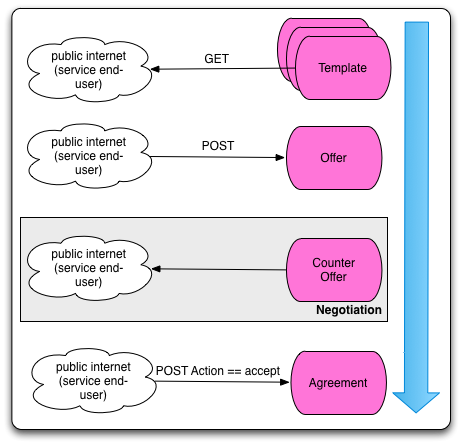
\includegraphics[width=60mm]{sla-occi-agreement.png}
\caption{\label{sla-agreement} SLA negotiation}
\end{figure}



Based on those 3 Categories the following scenario can be realized:(k)

\begin{enumerate}
\item The customer (from now on referred to as User) requests if the Agreement(l) kind, the Agreement link and available Templates (for SLOs and Metrics) are available in the service provider’s QI. The user can use all the query interface capabilities such as filtering to accomplish this job.
\item \verb|HTTP GET /.well-known/org/ogf/occi/|
\item The User tries creates an instance of the kind Agreement along with provided templates. This is known as the offer. If the service provider agrees with the offer it’ll return a 200/201(m) OK and create the Agreement. If the service provider chooses to reject Bad Request is returned. If the service provider wants to make a counter-offer 302 is used (This is part of the negotiation phase). A Location with a temporary agreement should be created
\item \verb|HTTP POST /agreement/| or \verb|HTTP PUT /agreement/123| (with Category agreement;scheme... and templates as Mixin definitions if applicable)
\item When the user finally wants to agree upon the agreement he needs to trigger the agree Action. The state of the agreement will change according the life cycle. Now resources can be put under this agreement.
\item \verb|HTTP POST /agreement/123?action=agree|
\end {enumerate}

{
\color{blue}
[k]Foued jrad:
The name of the action as defined in the agreement kind is "agree" .  Therefore action = accept can be changed to action = agree

[l]Andy Edmonds:
wouldn't the customer request to see if templates are available first (e.g. what have you in your shop?)?

Thijs Metsch:
he would - last sentence of point 1

Andy Edmonds:
any objections to changing the ordering of the sentence?

Thijs Metsch:
not at all - makes sense
[m]Alexander Papaspyrou:
What's the use case for 200?



Andy Edmonds:
200 would return a rendering of the Agreement in the body. A 201 would not, just the Location



Alexander Papaspyrou:
I guess 200 happens on PUT while 201 goes for POST. If so, this should be stated more clearly in the text.
}


\begin{enumerate}
\item Existing or newly created resources can now be bound to the agreement using the AgreeementLink.
\item \verb|HTTP POST /agreement/| (with Category of the resource and a link description)
\item \verb|HTTP POST /agreement/link/| (with Kind of the AgreementLink and source and target attributes)
\item \verb|HTTP POST /agreement/123| (with the Link definition)
\end{enumerate}

\begin{figure}
\centering
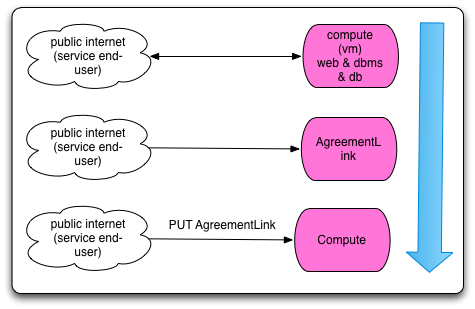
\includegraphics[width=10cm]{occi-sla-prov.png}
\caption{\label{slaprovisioning} SLA provisioning}
\end{figure}

\subsection{An Audit-Mixin}

This mixin allows for date stamping of certain operations related to SLA establishment, updates and termination.

\occitemplate
{date\_audit}
{\url{http://schemas.ogf.org/occi/audit\#}}
{Adds the date-time stamping to an associated instance}
{None}
{None}
{
\begin{tabular}{|l|l|l|l|l|} \hline
Attribute & Type & Multiplicity	& Mutability & Description \\ \hline
 	end & string & 0..1 & Mutable & ISO8601 (n) \\ \hline
 	created & string & 1 & Immutable & ISO8601 (n) \\ \hline
 	updated	& string & 0..1	& Immutable & ISO8601 (n) \\ \hline
\end{tabular} 
}

{
\color{blue}
[n]Andy Edmonds:
the addition of a decimal fraction to the smallest time unit if higher precision is needed. [ISO web site]
}

\section{Instance Monitoring (o)(p)}

{
\color{blue}
(o)Foued jrad:
The document discusses the monitoring of the running instances through metric mixins. But how the common provider monitoring data,which are not related to a specific instance (e.g location, resource capacity, toatal usage statistics) can be presented. Use case:  this kind of provider monitoring can be consumed by service brokers for SLA negotiation.

(p)Augusto Ciuffoletti:
If appropriate, one could add other strong motivations for monitoring, besides service level verification. E.g., user side resource optimization, process certifications, etc... It depends on whether you want an "how to" doc or a "why" doc. In the present statement it is unclear what a "potential problem" may be: failures should be managed by *aaS provider.
}

Once a service consumer has running instances with a provider, the next thing that this consumer should be able to do is monitoring those instances to proactively manage potential problems. As such—from a point of view of manageability—monitoring is essential. The approach taken in this monitoring extension is to keep things as simple as is possible and stay compatible with the Core model in that the defined Mixin can be validly applied to all instances of Entity.

\begin{figure}
\centering
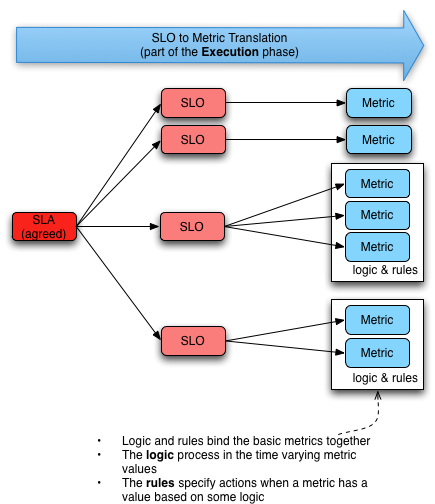
\includegraphics[width=10cm]{occi-sla-metric.png}
\caption{\label{slametric} SLA to metric transaction}
\end{figure}


\subsection{Note on Monitoring and SLAs}
Before continuing into the specification of monitoring, it is valuable to discuss how monitoring and SLAs are related. In order for a provider to offer SLAs, it needs to be monitoring his service instance offerings with respect to certain basic (e.g. network receive per second) and/or calculated metrics (e.g. uptime). Such metrics, expressed as SLOs (see figure below),(q) then form the basis of service offerings that the provider is willing to guarantee. Note that, these do not necessarily resemble the service provider’s internal representation of those SLOs. When a service consumer accepts an SLA for which the provider asserts he can satisfy the conditions, and the consumer creates service instances based on that Agreement, the service provider MUST setup the required monitoring on those instances so that the related metrics be collected and verified (through logic and rules) by internal SLA management systems of the provider. The service provider SHOULD, at a minimum,(r) expose to the consumer the SLA terms as monitorable metrics. The consumer COULD access these SLOs as metrics using the OCCI monitoring specification.

{
\color{blue}
[q]Alexander Papaspyrou:
Same as above: confusing regarding terminology.

Andy Edmonds:
SLO $\approx =$ metric

[r]Augusto Ciuffoletti:
Is there a need to specify that this is a minimum. Why not just a flashing led?
}

\subsection{Representing Metric}
A metric is represented by an instance of OCCI Mixin. A metric has a set of associated attributes. It should be kept in mind that a Metric is in effect an Attribute of the resource being monitored and so their formulation is very much the same as what is seen with X-OCCI-Attribute[s].



\subsection{Metric Mixin Definition[t]}

{
\color{blue}[t]Andy Edmonds:
Ideally a metric would be linked to an Attribute but as attributes are not 1st class entities in the model a relationship cannot be made, hence the "value" attribute
}

\occitemplate
{metric}
{\url{http://schemas.ogf.org/occi/monitoring\#}}
{A metric mixin}
{None}
{}
{
\begin{tabular}{|l|l|l|l|l|} \hline
Attribute & Type & Multiplicity	& Mutability & Description \\ \hline
	value & string & 1 & Immutable & \parbox{2in}{Based on unit, infer the value’s type.}  \\ \hline
	timestamp & string[n] & 1 & Immutable & ISO8601 [n] \\ \hline
	samplerate & float & 0..1 & Mutable & hertz?[u] \\ \hline
	resolution & string & 0..1 & Mutable & SI prefix \\ \hline
	unit & string & 1 & Immutable & \parbox{2in}{If the metric being monitored is an OCCI attribute (e.g. occi.compute.memory) then the designated unit is used. Otherwise, use provider defined appropriate unit.[v]}\\ \hline
\end{tabular} 
}

{
\color{blue}
[u]Victor Bayon:
Updates/Minute? Herzt is probably too small

Andy Edmonds:
Yes good point. n updates per second is probably the lowest unit we want to deal in

Alexander Papaspyrou:
Alas, updates per second is not very different from Hertz...

Andy Edmonds:
Problem with hertz is that to specify an update every hour is inconvenient to represent in hertz: 0.000277778 hertz

Alexander Papaspyrou:
Yup. I don't really care, as long we allow SI units (m/ki/Mi/Gi/Ti etc.) for expressing the order of magnitude.

[v]Andy Edmonds:
hint to implementor
}


\subsection{Example Metric Mixins}

\subsubsection{Compute Metrics}
Compute Metrics Available in prototype:
\begin{itemize}
\item {\tt cpu.user, cpu.sys, cpu.wait, cpu.lavg1, cpu.intsec, cpu.ctxsec,}
\item {\tt mem.tot, mem.buf, mem.used, mem.free, mem.cached, mem.swap}
\end{itemize}


These all MUST have their rel attribute set to \verb"http://schemas.ogf.org/occi/monitoring#metric"

\begin{tabular}{|l|l|l|}
Title & Term & Scheme \\ \hline
cpu.user & user & \url{http://iolanes.eu/occi/infrastructure/metric/compute/cpu\#} \\ \hline
cpu.sys & sys & \url{http://iolanes.eu/occi/infrastructure/metric/compute/cpu\#} \\ \hline 
cpu.wait & wait & \url{http://iolanes.eu/occi/infrastructure/metric/compute/cpu\#} \\ \hline
cpu.lavg1 & lavg1 & \url{http://iolanes.eu/occi/infrastructure/metric/compute/cpu\#} \\ \hline
cpu.intsec & intsec & \url{http://iolanes.eu/occi/infrastructure/metric/compute/cpu\#[w]} \\ \hline
cpu.ctxsec & ctxsec & \url{http://iolanes.eu/occi/infrastructure/metric/compute/cpu\#} \\ \hline
mem.tot & tot & \url{http://iolanes.eu/occi/infrastructure/metric/compute/memory\#} \\ \hline
mem.buf & buf & \url{http://iolanes.eu/occi/infrastructure/metric/compute/memory\#} \\ \hline
mem.used & used & \url{http://iolanes.eu/occi/infrastructure/metric/compute/memory\#} \\ \hline
mem.free & free & \url{http://iolanes.eu/occi/infrastructure/metric/compute/memory\#} \\ \hline
mem.cached & cached & \url{http://iolanes.eu/occi/infrastructure/metric/compute/memory\#} \\ \hline
mem.swap & swap & \url{http://iolanes.eu/occi/infrastructure/metric/compute/memory\#}  \\ \hline
\end{tabular}

{\color{blue}
[w]Victor Bayon:
intsec = Interrupts/Second
ctxsec = ContextSwitch/Sec
}

\subsubsection{Network Metrics(x)}
Network Metrics Available in prototype:
1. net.rxkbtot, net.txkbtot

{
\color{blue}
(x)Augusto Ciuffoletti:

The network metrics that are given in the draft are oriented to network interfaces, which can be considered as part of a computing device, and might be consistently indicated in this kind of mixin.

Instead network metrics should measure performance of networking resources, whatever they are. Typical metrics are point to point roundtrip times, gateway throughput, link bandwidth for an L2 device. Since one such type is defined in the “infrastructure” document, I’d better start with bandwidth, or a maximum RTT (which includes NICs characteristics), or packet loss rate etc.
}

\begin{tabular}{|l|l|l|}
Title & Term & Scheme \\ \hline
net.rxkbtot & rxtot & \url{http://iolanes.eu/occi/infrastructure/metric/network\#} \\ \hline
net.txkbtot & txtot & \url{http://iolanes.eu/occi/infrastructure/metric/network\#} \\ \hline
\end{tabular}

\subsubsection{Storage Metrics}
Storage Metrics Available in the prototype:
1. dsk.readtot, dsk.writetot, dsk.readkbtot,dsk.writekbtot


\begin{tabular}{|l|l|l|}
Title & Term & Scheme \\ \hline	
	dsk.readtot & readtot & \url{http://iolanes.eu/occi/infrastructure/metric/storage\#} \\ \hline
	dsk.writetot & writetot & \url{http://iolanes.eu/occi/infrastructure/metric/storage\#} \\ \hline
	dsk.readkbtot & readkbtot & \url{http://iolanes.eu/occi/infrastructure/metric/storage\#} \\ \hline
	dsk.writekbtot & writekbtot & \url{http://iolanes.eu/occi/infrastructure/metric/storage\#} \\ \hline
\end{tabular}

\subsection{Monitoring Behaviour[y]}

{
\color{blue}
[y]Andy Edmonds:
It is likely this is incomplete - inputs appreciated
}

\subsubsection{Discovery of Metrics}

Sample Query Interface Rendering of Two Metrics offered by the provider

\begin{verbatim}
> GET /-/ HTTP/1.1        


...
< Category: metric; scheme=”http://iolanes.eu/occi/infrastructure#”[z]; class=”mixin”; title=”The metric mixin”; attributes=”timestamp{immutable} samplerate resolution unit”
< Category: rxtot; scheme=”http://iolanes.eu/occi/infrastructure/metric/network#”; class=”mixin”; title=”net.rxkbtot”; attributes=”timestamp{immutable} samplerate resolution unit”; rel=”http://iolanes.eu/occi/infrastructure#metric”; location=”/metric/network/rxtot”
< Category: user; scheme=”http://iolanes.eu/occi/infrastructure/metric/compute/cpu#”; class=”mixin”; title=”cpu.user”; attributes=”timestamp{immutable} samplerate resolution unit”; rel=”http://iolanes.eu/occi/infrastructure#metric”; location=”/metric/compute/cpu/user”
…
\end{verbatim}

{
\color{blue}
[z]Foued jrad:
I think it is better to use the introduced scheme \url{http://schemas.ogf.org/occi/monitoring#} for the sample.
}

\subsubsection{Activate Specific Metrics[aa]}

{
\color{blue}
[aa]Andy Edmonds:
parameterise this metic provisioning e.g. sample frequency, resolution etc
}

Add a mixin[ab]

{
\color{blue}
[ab]Andy Edmonds:
How to activate all applicable metrics?

Andy Edmonds:
probably not a good idea. number of metrics per resource could be potentially large (e.g. number of dtrace probes on mac os x is > 240k)

Alexander Papaspyrou:
This leads us again into issues with header sizes, actually.

Andy Edmonds:
recommend JSON to the rescue
}

\begin{verbatim}
> PUT[ac] /$RESOURCE/123-123-123


> category: rxtot; scheme='http://iolanes.eu/occi/infrastructure/metric/network#'; class='mixin'
> category: user; scheme='http://iolanes.eu/occi/infrastructure/metric/compute/cpu#'; class='mixin'
\end{verbatim}

\subsubsection{Update (configure) specific Resource Metric Parameters}

By saying update, we mean to update the attributes of the metric and not the values that they represent. Only those metric attributes that are signalled as mutable can be modified.
Full Update
\begin{verbatim}
> PUT /$RESOURCE/123-123-123
\end{verbatim}

Partial Update
\begin{verbatim}
> POST /$RESOURCE/123-123-123
\end{verbatim}

\subsubsection{Deactivate specific[ad] Resource Metric}

{
\color{blue}
[ad]Andy Edmonds:
Deactivate all metrics?

Andy Edmonds:
the same PUT but without the metric mixins
}

PUT the resource representation without those metrics to be deactivated.
\begin{verbatim}
> PUT /$RESOURCE/123-123-123


< category: occi.compute.memory; scheme='http://iolanes.eu/infra/metrics#'; class='mixin'
< category: occi.compute.speed; scheme='http://iolanes.eu/infra/metrics#'; class='mixin'
\end{verbatim}

\subsubsection{Retrieve a Instantaneous Metric Value}
\begin{verbatim}
> GET /service/123-123?attribute=occi.service.messages.throughput[ae]
< 204 OK HTTP/1.1
…
< x-occi-attribute: occi.service.messages.throughput=2.0
\end{verbatim}

{
\color{blue}
[ae]Andy Edmonds:
this is just a simple example
}


alternative:
\begin{verbatim}
> GET /compute/123-123-123
> Category: occi.service.messages.throughput; scheme='http://iolanes.eu/infra/metrics#'; class='mixin'

< x-occi-attribute: occi.service.messages.throughput = 2.0
\end{verbatim}
\subsubsection{Retreive all[af] Instantaneous Metric Values}
{
\color{blue}
[af]Andy Edmonds:
There will be an issue with this where number of metrics on a resource  is large - HTTP header overflow. Suggest that JSON is preferred here.
}

\begin{verbatim}
> GET /service/123-123
< 200 OK HTTP/1.1
< Category: occi.service.messages.throughput; scheme='http://iolanes.eu/infra/metrics#'; class='mixin'
<
< x-occi-attribute: occi.compute.memory = 2.0
< x-occi-attribute: occi.compute.cores = 2
< x-occi-attribute: occi.service.messages.throughput = 2.0
\end{verbatim}

\subsubsection{Response Content as CSV[ag][ah]}

{
\color{blue}
[ag]Victor Bayon:
could be the output be different (e.g. a png)?

[ah]Andy Edmonds:
Useful, simple format for "data scientists"
}

\href{http://dl.dropbox.com/u/165239/sampleCSVData4OCCIMonitoringInterface.csv}{Sample data file} Content-type: text/csv

\subsubsection{Monitoring Push[ai] Notification[aj]}

{
\color{blue}
[ai]Augusto Ciuffoletti:
This is a very important feature. Overall, instantaneous values (see above) are of little value: as a general rule one prefers robust indicators, like weighted averages and such. But the user may appreciate the availability of the full history, and the provider cannot host (not for free, anyway) the quantity of data collected while monitoring. So it may be of interest to send data directly to the user. But an html (or SOAP) based transfer of this kind may have a heavy footprint. One alternative is to send data using a transport level stream (RTP). How does this sound?
[aj]Andy Edmonds:
TODO - solve this and we've a significant differentiator
}

\begin{itemize}
\item What about the use of streamed HTTP traffic e.g. how node.js does some streaming operations for output? 
\item Can a client can signal their preference?
\end{itemize}

\section{Proposed changes[ak] to the OCCI specification}

{
\color{blue}
[ak]Alexander Papaspyrou:
In the process of making changes to HTTP, we could also do partial retrieval/update.

Andy Edmonds:
and likely review content types/negotiation
}

\begin{itemize}
\item Alter the Query Interface so default values can be defined for templating
\item  add default value and include enums
\item  Add Notification mechanisms (look at SNIA’s DDMI)
\item Also to chunked transfer encoding
\end{itemize}

\newpage
\hrulefill

{
\large
\bf
\color{red}
Below this line are our thoughts and bullet points - trying to get this all into a ‘real’ doc
}

\hrulefill


Considerations



\begin{tabbing}
0000\=0000\=0000\=0000 \kill
Eh? WS agreement? why? :) \\
	\>We should take a lokk at WSAG-Negotiation draft - WSAG spec itself has too much SOAP \\
	\>	\>Take the model! \\
	\>States to be supported: \\
\end{tabbing}

\begin{figure}
\centering
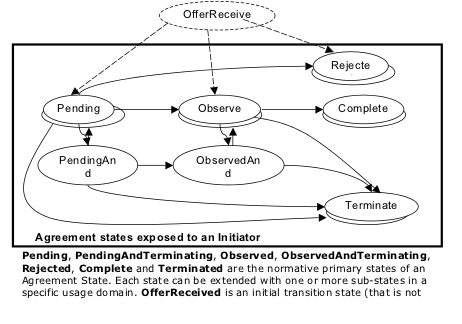
\includegraphics[width=10cm]{states.png}
\caption{\label{states} Agreement states exposed to an Initiator}
\end{figure}
	
\begin{tabbing}
0000\=0000\=0000\=0000 \kill	
	\>SLA@SOI SLA model \\
	\>Link resource to agreement implies monitoring \\
	\>	\>monitoring a requirement \\
	\>Example: verify that it is an 800MHz machine with an apache server with latency of 300ms \\
	\>	\>Latency of the webserver -> how are you going to check that?, latency from where? the client?  \\
	\>Applicable to hardware and software levels: \\
	\>	\>e.g. negotiate a VM running Apache \\
	\>Provisioned resource is linked to agreement \\
	\>WS-Agreement could be used as the content. OCCI attributes could be used within qualified by the OCCI namespace \\
	\>Extend mixins to allow for type and value info so that a resource template mixin can be used as the basis of a SLA template \\
	\>Big bonus points for all this expressed as ABNF \& ANTLR \\
	\>With the current setup we could let fall several resource instances, of different kinds, fall under one agreement - cool :-) \\
	\>What’s the purpose of the SLA once agreed. Will it have rules or “smarts” to proactively resolve SLA violations? Or will it only report that a violation occurred and the provider executed counter-measures? Will the user have the option to specify their own violation counter-measures? \\
\end{tabbing}


\section*{Terminology}

\begin{longtable}{|p{2cm}|p{11cm}|p{3cm}|}
Term	& Definition	& Representation in OCCI SLA \\ \hline
SLA & 
\parbox{3in}{An agreement defines a dynamically-established and dynamically managed contract/agreement between between a service provider and a customer.} &
\parbox{1in}{An agreement resource instance and a set of (1...*) resource instances linking to it} 
\\ \hline
from SLA\@SOI &
\begin{minipage}{11cm}
\begin{enumerate}
\item An agreement defines a dynamically-established and dynamically managed relationship between parties. The object of this relationship is the delivery of a service by one of the parties within the context of the agreement. The management of this delivery is achieved by agreeing on the respective roles, rights and obligations of the parties. The agreement may specify not only functional properties for identification or creation of the service, but also non-functional properties of the service such as performance or availability. Entities can dynamically establish and manage agreements via Web service interfaces. (source: WSAgreement)
\item An Agreement between a service provider and a customer. The SLA describes the service, documents service level targets, and specifies the responsibilities of the service provider and the customer. A single SLA may cover multiple services or multiple customers. (source: ITIL)
\item A Service Level Agreement (SLA) is an element of a formal, negotiated contract between two parties, viz., a Service Provider (SP) and a Customer. It documents the common understanding of all aspects of the service and the roles and responsibilities of both parties from service ordering to service termination. (source: SLA Management Handbook, TMForum) A single SLA may cover simple or compound services, or multiple customers. SLAs may be dynamic. Dynamic SLAs include one or more parameters that are variable. These variable parameters may be associated with agreed pricing scales.
\end{enumerate}
\end{minipage}
& 
\\ \hline
Agreement & 
A set of terms (reflected in a resource instances) on which the client and service provider ‘agree’ (Part of an SLA) &
An resource instance of ind Agreement - For example:
http://example.com/agreement/123
(Kind: Agreement, Mixin=*{Template Mixin}, Attributes=(see monitoring))
\\ \hline
Negotiation &
The process of creating an agreement &
Creation of an agreement instance:
HTTP POST/PUT http://example.com/agreement/
\\ \hline
Template &
An agreement template is a representation used by the agreement responder to advertise the types of requests it is (possibly) willing to accept/handle. &
Through a Mixin (very much in the style of resource template mixins [infrastructure spec]) - For example:
\verb|Category: gold; scheme="http://"; class="mixin"; attributes="occi.compute.memory{value=1, type='int', immutab|
\\ \hline	
from SLA\@SOI  & 
Glossary &
An agreement template is a (XML) document used by the agreement responder to advertise the types of offers it is willing to accept. (source: WSAgreement)        
\\ \hline
\end{longtable}	

	

\section*{Open Issues}
\begin{itemize}
\item How to ensure that resource instances have needed monitoring mixins assigned?
\item What goes into kind agreement, agreement link, and actions, attribtues needed?
\item What’s with the history of an agreement? (aka. Agreement violated 2 days ago?)
\end{itemize}


\section*{Flow of Resource Acquisition}
\begin{enumerate}
\item Negotiate: retrieve SLA templates. Populate suitable template with required values.
  \begin{itemize} 
  \item Simple case of “Negotiation” is to provision - binary decision (yes or no)
  \end{itemize}
\item Agree: result of client accepting negotiated template instance.
  \begin{itemize} 
  \item Are resources reserved at this stage?
  \item If a client wants to cancel before the execution stage they can issue a DELETE on teh template instance ID.
  \end{itemize}
\item Execute: signal to provision the associated resources. Provisioned resources are linked to the template instance.
\item Monitor and Notify: Part of the provisioning process configures monitoring of the resources
  \begin{itemize} 
  \item There are monitoring directives contained in the SLA that need to be translated (ugh) to a spec the monitoring system understands - might be some ANTLR skills are called for :p
  \end{itemize}
\end{enumerate}

This maps to the flow of agreement that is in SLA@SOI where they query, reserve and execute. See \href{http://dl.dropbox.com/u/165239/query-reservation.pptx}{this presentation as an overview}.

\begin{itemize}
   \item POST agreement template to service: service instance location not important
   \item PUT agreement template to service: service instance location is important and must be known in advance
   \item An agreement instance can be associated with many service instances
   \begin{itemize}
   \item What impact does this have on subsequent provisionings and provider capacity?
   \end{itemize}
\end{itemize}

\section*{Negotiation of Agreements}
Uses the stuff defined before...
\subsection*{Kind definitions}
{\bf Agreement} \\
An agreement itself... \\
{\bf AgreementLink} \\
Used to link a resource instance to an agreement... \\
{\bf Template Mixins} \\
Plantinum, Gold, Silver etc... \\

\section*{Negotiation process}

\begin{figure}
\centering
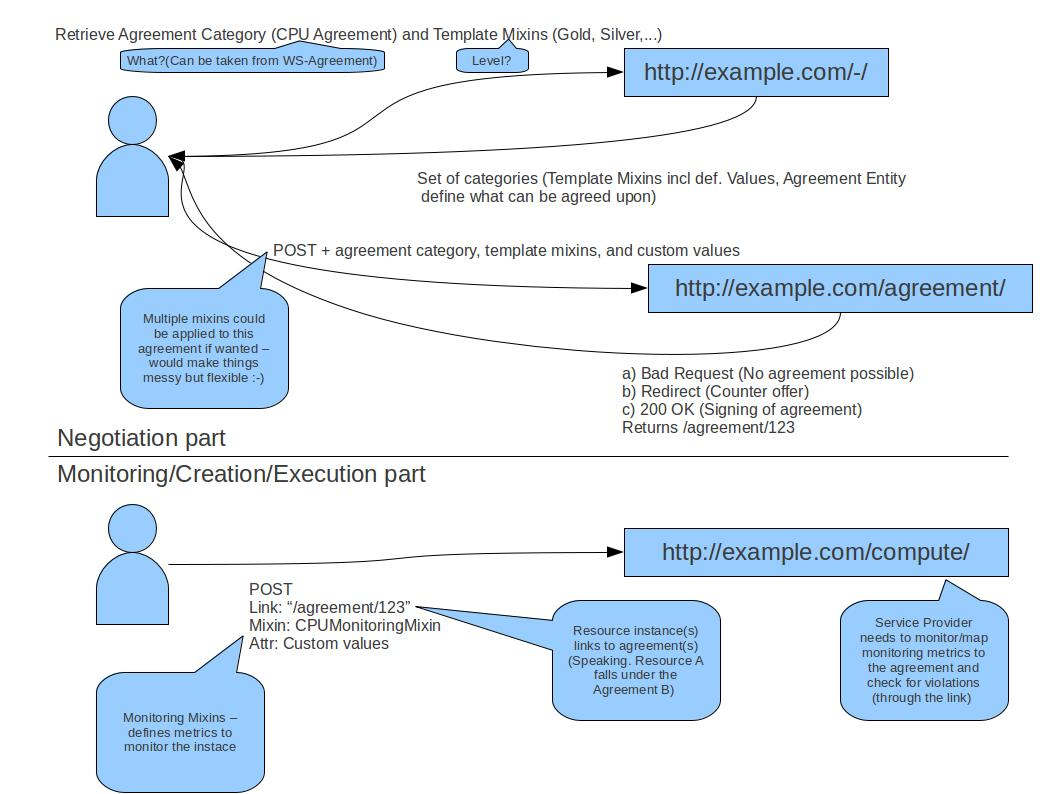
\includegraphics[width=100mm]{negotiationProcess.jpg}
\caption{\label{negotiationprocess} The negotiation process}
\end{figure}

   1. (Optional) - Retrieve a set of template mixins through the Query interface

\begin{verbatim}
> GET /-/
< Category: gold; scheme="http://"; class="mixin"; attributes="occi.compute.memory{value=1, type='int', immutable, required}"
\end{verbatim}

\begin{enumerate}
\item  Create a new resource instance of kind Agreement:
   \begin{enumerate}
	\item Request MUST include: Agreement Kind
	\item MAY include Mixins from the templates (like GOLD)
	\item MAY include additional/changed values to agree upon (Customization)
   \end{enumerate}
\item  Service can respond:
   \begin{enumerate}
	\item with 200 OK and accept the agreement
	\item redirect to a counter over
	\item Bad Request and not accept the agreement
   \end{enumerate}
\item  Client can now link to this agreement (Semenatics: add 1...* resource instances to an agreement)
   \begin{enumerate}
	\item Link must be of kind AgreementLink (rel is therefore: Agreement kind)
	\item Link can be added to an existing resource instance, or to a new one
   \end{enumerate}
\item  Service provider needs to take care that the resource instance linked to an agreement
   \begin{enumerate}
	\item have the right mixins so they can be monitored
	\item monitor the resource instances an check against agreed values
	\item report states (see state diagram)[al]
   \end{enumerate}
\end{enumerate}

{
\color{blue}
[al]Thijs Metsch:
Notification would be cool here

Thijs Metsch:
Also History?

Andy Edmonds:
Notifications will require some sort of rule system. Currently, for monitoring we've only considered a basic rule capability. I would imagine that for SLAs a more complex rule system is needed but one that can build upon the monitoring systems. Might be worth having a look at the SLA@SOI model? History of the metrics is part of the monitoring system.

Thijs Metsch:
Have seen that - was just wondering if same could apply here (technical speaking)
}


{
\color{green}
Execution of Agreement
TODO
Representing Calculated Metrics
Calculated metrics appear as raw metrics associated with a Resource. A calculated metric is the output of a Processor Resource. A Processor Resource represents the entity (e.g. software entity) that applies a function on 1 or more inputs. A Processor Resource has one or more raw inputs (Defined by mixin metrics). A Processor Resource has one output. A Processor Resource is linked to a Metric. When the system (implementation) reads a Processor it returns the calculated value. This allows the calculated value be offered as a Metric associated with a monitored Resource. If the Metric is a calculated metric then the mixin definition of that Metric will have its rel value pointing to the Processor Resource type (kind) e.g.

\begin{verbatim}
category: occi.core.cpu.cost; scheme=”http://schemas.ogf.org/occi/metric#”; class=”mixin”; rel=”http://schemas.ogf.org/occi/processor#cpu_billing_calculator”
\end{verbatim}

Only a single rel value is needed if processors can be represented as a graph of collaborating processors with the sole purpose of outputting a single value which is used as the “raw” metric value. This would follow a similar approach taken with WS-BPEL where the internal interfaces that make up the composition are of no concern to the client but only the “terminal” external interface.
Definition of Metric Mixins
Here a set of definitions for metrics Mixins would be cool (Maybe copy from WSAG-Negotiation)? Would be very useful to have WSAG mappings to OCCI mixins. In the current planned prototype the following metrics will be available:


how to have specify an instance’s subresources in a category?
suggestion:
\begin{verbatim}
< category: speed; scheme='http://iolanes.eu/infra/metrics#'; class='mixin'; location=”/compute/{occi.core.id}/metric/speed”
\end{verbatim}

Metric attribute defaults in QI
sample rate, resolution, simple type, unit (rate, unit - from ganglia/rrdtool)


Metric history should be maintained - the duration is subject to SLA
Deactivate all Resource Metrics
\begin{verbatim}
> DELETE /$RESOURCE/123-123-123


< category: occi.compute.*; scheme='http://iolanes.eu/infra/metrics#'; class='mixin'
\end{verbatim}


Metric history should be maintained - the duration is subject to SLA


Retrieve a Ranged Metric Value
Could we slightly abuse the content-range header? Specify a start and end timestamp as the value for the time range?
\begin{verbatim}
> GET /compute/123-123-123
> category: occi.compute.cpu.user; scheme=’http://’; class=’mixin’
> x-occi-attribute: occi.compute.cpu.user.rangefrom=897777337
> x-occi-attribute: occi.compute.cpu.user.rangeto=897788888


< ???
\end{verbatim}

Inline
\begin{verbatim}
> GET /compute/123-123-123/metric/cpu/user?rangeFrom=XXX&rangeTo=XXX
\end{verbatim}
Retrieve a Set of Metrics
Multipart? CSV
Retrieve a Metric Group
A metric group is defined by a tag. If 2 or more metrics are associated with a tag then they’re deemed to be a metric group. Two modes: X-OCCI-Location or inline data.
}

\section*{Considerations}
\begin{itemize}
\item other monitoring providers: amazon cloud watch, cloudkick, pingdom, See XDR in ganglia, however there is a problem with ganglia data definition. It defines a very flexible data format, but once is running everything is static, cannot change its configuration, ends up being too verbose. 
\item monitoring designed as an OCCI mixin
\item An entity has a set of Metrics
\item A metric is related to an Attribute[am]

{\color{blue}
[am]Andy Edmonds:
How to relate
?

Andy Edmonds:
@tmetsch@gmail.com any ideas on this?
}

\item A Metric has a set of rules threshold values
\item A Rule is related to a Metric and/or other rule (this will be tricky)
\item Types (e.g Float, Integer, String, etc) 
\item Are the OCCI types should be enough? YES
\item string, int, float, enum, boolean
\item Units: if the metric being monitored is an OCCI attribute (e.g. occi.compute.memory) then the designated representational occi type (string, enum, integer, float, boolean) is used. Otherwise, use provider defined appropriate representational occi type.
\item It is likely better to link the metric to the attribute rather than duplicate this info
\item Static versus dynamic (number of CPUs is not going to change rapidly per resource but CPU load yes) - sample rate defines this - it’s fast (dynamic) or slow moving (static)
\item metric resolution - magnitude (mega, giga, tera etc) and significant decimal places, readonly
\item storage period (this could be also resampling rates per period of time, like RRDs)
\item What about modification of these types?
\item Depends on the client implementation
\item Client defined sample rate? Yes, a provider can reject the value however.
\item Metric data range - parameters to a URL request. start, stop dates as timestamps (unix, ISO format)
\item Push Notifications?
\item Metric validity: On the service side, how long the metric is/could be valid for (e.g. 30 seconds), as it is the client will be the one pushing the updates. After that time the metric value is invalid.
\item the system will issue a timestamp with the metric value so valid time is timestamp + metric sample rate.
\item Add metrics by linkage using OCCI Link between a Resource and Metric? NO Metric is a mixin
\item Metric groups? could be done with OCCI tags (user mixin), not mandatory but capability exists already in core spec
\item Rules and alerts - need to be related to SLA. Only have thresholds - breaking a threshold sends a message to another system for further processing [an](that when a threshold was exceeded, a user defined message could be sent).  Rules are a can of worms, as there their definition could be very complex (e.g. time domain, event based, correlation, aggregation, etc).
{
\color{blue}
[an]Andy Edmonds:
Look to use CDMI Queues here
}

\item an import interface? not in the spec, for now a provider concern.
\item In general, for metrics it may not be useful to offer a standardised set of metrics (given the large amount of possible metrics that could be offered) but rather we should specify a way that any metric fitting the metric model can be understood by a client.
\item User defined metrics?
\end{itemize}

{
\color{green}
\section*{Required OCCI Extensions}
OCCI Mixin Extension
   1. It is an extension to Category
   2. Allow for type and value info so that a resource template mixin can be used as the resource template e.g.
   3. Needed by SLA templates and resource template mixins to be complete




Category: gold; scheme="http://"; class="mixin"; attributes="occi.compute.memory{defaultvalue=1, type='int', immutable}"


   1. Also requirement to advertise enum values
OCCI Filter Extension
   1. Needed by monitoring. Allow for wild cards in the filter e.g.
\begin{verbatim}
GET /-/
> category: *; scheme=”http://schemas.ogf.org/occi/infrastructure/metric#”; class=”kind”
\end{verbatim}
}

\section*{Resources}
\begin{enumerate}
\item WSAG Specification:  \url{http://ogf.org/documents/GFD.107.pdf}
\item Paper on restyfing WSAG: \url{http://www.ws-rest.org/2011/proc/a12-kubert.pdf}
\item A student’s master thesis: Source N/A
\item SLA@SOI presentation: \url{http://dl.dropbox.com/u/165239/query-reservation.pptx}
\item WSAG Negotioation draft: \url{http://forge.gridforum.org/sf/docman/do/listDocuments/projects.graap-wg/docman.root.current_drafts.ws_agreement_negotiation_specifi}
\end{enumerate}


\subsection*{Attic}

I would love to see the following:
\subsubsection*{CostsMixin[ao]}

{
\color{blue}
[ao]Andy Edmonds:
Is this better suited to a billing interface?

Andy Edmonds:
Costs are calculated metrics. Currently the only consideration for metrics are "raw" metrics that are exposed by the resource and that there is a 1:1 mapping of resource attributes (e.g. occi.compute.memory) to metric

Thijs Metsch:
If we define it that we - we should move it...what would be a reason for only allowing raw values? E.g. I'm thinking of MIPS, latency of a service  - that'll be calculated too

Andy Edmonds:
if you have calculated metrics the complexity of the current monitoring interface may increase.
however that doesn't mean that the current interface as defined can't offer other metrics
occi.compute.cpu.user, occi.compute.cpu.cost
occi.compute.cpu.cost would be then linked to some aspect of a billing model/interface.
in that sense, although it's calculated elsewhere, occi.compute.cpu.cost is raw

Thijs Metsch:
the idea of defining the metrics not so much bound to the kinds of resource instance(s) is the reusability - but maybe this only applies to this billing mixin, and should be moved to a billing extension :-) (raw vs. calculated this is a point of discussion I guess).

Thijs Metsch:
Also: what would be the costs/work to extend the complexity of the metrics interface to support this?

Thijs Metsch:
costs stuff should be moved to billing ext.
}


This can now be supported as a calculated metric (derived)

Definition:
\begin{enumerate}
\item costs;\verb|scheme=http://schemas.ogf.org/occi/billing|;
\end{enumerate}

Attributes:
\begin{enumerate}
\item accumulate\_costs (int)
\item costs\_per\_timeframe (int)
\item timeframe (long) in sec
\item currency (enum [\$, EUR)]
\end{enumerate}

Actions:
\begin{enumerate}
\item N/A
\end{enumerate}

\end{document}
